\chapter{Peripheral Driver Development (1)}
\label{Chap:peripheral_driver_1}

\section{Introduction}

The structure of \autoref{Chap:peripheral_driver_1} is illustrated in \autoref{fig:driver_part_1:chapter_struct}.

\begin{figure}[h]
\centering
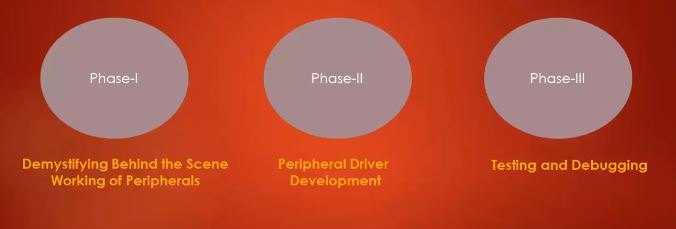
\includegraphics[scale=0.5]{Figures/driver_part_1/chapter_struct}
\caption{Chapter Structure}
\label{fig:driver_part_1:chapter_struct}
\end{figure}

\begin{itemize}
    \item Part 1 focuses on understanding the internal workings of key peripherals, such as GPIO and communication protocols like SPI.
    \item Part 2 covers the development of driver header files.
    \item Part 3 presents sample applications for each driver, including testing and debugging with a logic analyzer.
\end{itemize}

\underline{Bonus:} Guidance on installing and working with development tools, such as KEIL Microvision.

\newpage
\section{Debugging Techniques}

Before starting peripheral development, we will review several debugging techniques, as illustrated in \autoref{fig:driver_part_1:debug_techniques}.

\begin{figure}[h]
\centering
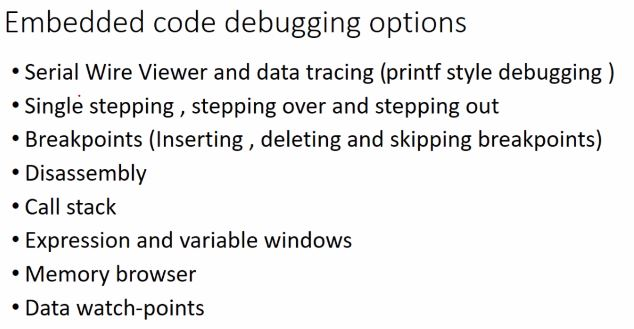
\includegraphics[scale=0.5]{Figures/driver_part_1/debug_techniques}
\caption{Different Debugging Techniques}
\label{fig:driver_part_1:debug_techniques}
\end{figure}

Each technique will be discussed in the following sections.

\subsection{Debugging General Steps}

\underline{General Rule:} To use any debugging technique shown in \autoref{fig:driver_part_1:debug_techniques}, we first need to \tbi{switch to debugging mode}. This is done by:

\begin{itemize}
    \item Building the project. Right-click, then select \verb|Debug as| $\rightarrow$ \verb|Debug as stm32 Cortex M application|.


    \item The window will switch to what is known as the \tbi{debug perspective}, as shown in \autoref{fig:driver_part_1:debug_perspective}.

\begin{figure}[h]
\centering
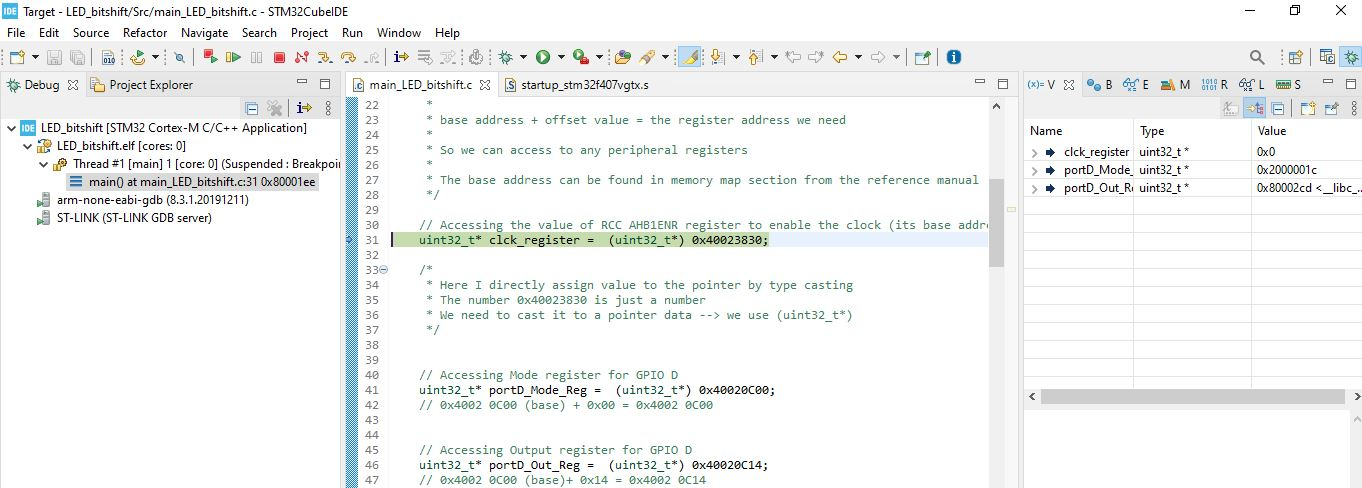
\includegraphics[scale=0.5]{Figures/driver_part_1/debug_perspective}
\caption{Editor Switched to Debug Mode}
\label{fig:driver_part_1:debug_perspective}
\end{figure}

    \begin{itemize}
        \item Notice the highlighting at line 31: this indicates that the code execution is currently at this line.
    \end{itemize}


\newpage

\item In \autoref{fig:driver_part_1:debug_perspective}, we can switch between debugger mode and editor mode. To return to editor mode, click on \verb|C/C++| as shown in \autoref{fig:driver_part_1:debug_mode_to_editor_mode}.

\begin{figure}[h]
\centering
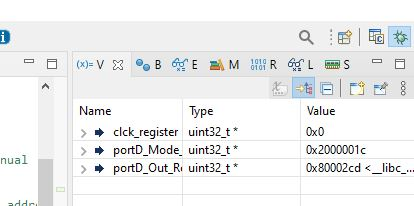
\includegraphics[scale=0.5]{Figures/driver_part_1/debug_mode_to_editor_mode}
\caption{Switching Back to Editor Mode}
\label{fig:driver_part_1:debug_mode_to_editor_mode}
\end{figure}

\item \underline{Assembly Code}: To view the equivalent assembly code of the \verb|C| code (for example, line 31 in \autoref{fig:driver_part_1:debug_perspective}), go to the \verb|Window| tab, then \verb|Show View| $\rightarrow$ \verb|Disassembly|.

A new mini window will appear (shown in \autoref{fig:driver_part_1:debug_mode_assembly}) on the right-hand side, displaying the Arm assembly instructions for the \verb|C| code.

\begin{figure}[h]
\centering
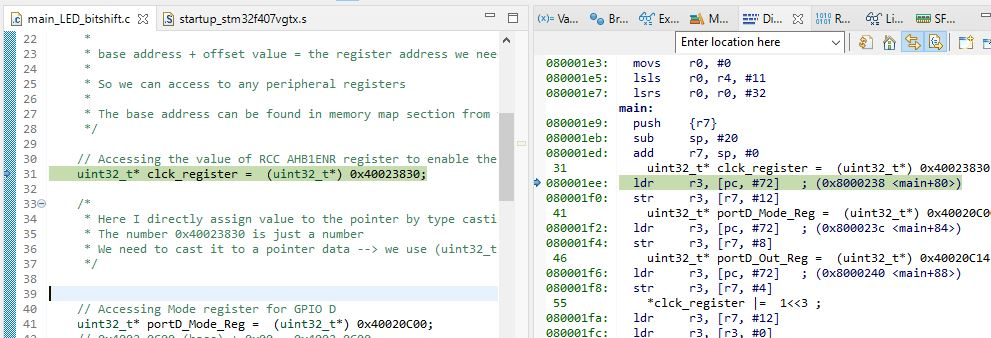
\includegraphics[scale=0.5]{Figures/driver_part_1/debug_mode_assembly}
\caption{Debug Mode: Displaying Assembly Instructions}
\label{fig:driver_part_1:debug_mode_assembly}
\end{figure}


    \begin{itemize}
        \item Notice that in the disassembly window, we first see the \verb|C| code, followed by the equivalent Arm assembly code.
    \end{itemize}

\item \underline{Alternating between Debug and Editing Mode:} On the right-hand side of \autoref{fig:driver_part_1:debug_perspective}, we have what is called the \tbi{debug view}, where all the functions called by our code are listed.
    
\end{itemize}

\newpage
\subsection{Stepping Options}
\label{Sub:peripheral_dev_1:Stepping_Options}

Stepping refers to line-by-line execution of the \verb|C| code (and not the assembly code, since one \verb|C| code line is generally equivalent to many assembly instructions). We have three options for stepping, as shown in \autoref{fig:driver_part_1:debug_stepping_options}.

\begin{figure}[h]
\centering

\includegraphics[scale=0.9]{Figures/driver_part_1/debug_stepping_options}
\caption{Debug Mode: Stepping Options}
\label{fig:driver_part_1:debug_stepping_options}
\end{figure}

\begin{itemize}
    \item Step Into: Enter the statement (e.g., go inside the function).

    \item Step Over: Execute one \verb|C| statement (e.g., execute a function without stepping into it).

    \item Step Return: Return from the function.
  
\end{itemize}


\subsection{Assembly Code Debugging}

To execute assembly-level code instead of \verb|C| code, follow these steps:

\begin{enumerate}
    \item Display the assembly window as described earlier:

    \begin{itemize}
        \item Go to the \verb|Window| tab, then \verb|Show View| $\rightarrow$ \verb|Disassembly|.
    \end{itemize}

    \item Activate instruction-level code by clicking the 'i' icon, as shown in \autoref{fig:driver_part_1:debug_assembly_activation}.

\begin{figure}[h]
\centering
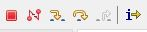
\includegraphics[scale=0.9]{Figures/driver_part_1/debug_assembly_activation}
\caption{Debug Assembly Mode: Activating Instruction Level Code}
\label{fig:driver_part_1:debug_assembly_activation}
\end{figure}

\item Then use the same stepping options explained in \ref{Sub:peripheral_dev_1:Stepping_Options}.
    
\end{enumerate}

\underline{Analyzing Assembly Window}: Let's take, for example, the assembly code shown in \autoref{fig:driver_part_1:debug_mode_assembly}.

\begin{itemize}
    \item On the right side, we see the \textit{addresses}: this indicates that this instruction is stored at this memory address. The memory type here is flash memory (used to download our code).

    \item These instructions are not stored in a textual way; they are stored as \textit{opcode}. To see the opcode, right-click on the assembly instruction, then click on \verb|Show Opcode|. For example, the opcode for 
    \autoref{fig:driver_part_1:debug_mode_assembly} is shown in 
    \autoref{fig:driver_part_1:debug_assembly_opcode}.

\newpage
\begin{figure}[h]
\centering
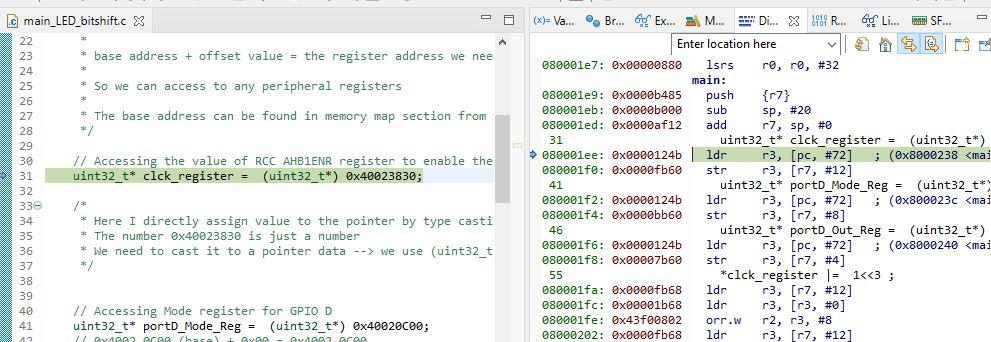
\includegraphics[scale=0.5]{Figures/driver_part_1/debug_assembly_opcode}
\caption{Debug Assembly Mode: Showing the Opcode of \autoref{fig:driver_part_1:debug_mode_assembly}}
\label{fig:driver_part_1:debug_assembly_opcode}
\end{figure}

    \item If we want to see the content of the registers, we can go to the \verb|Window| tab, $\rightarrow$ \verb|Show View|  $\rightarrow$ \verb|Registers|.

    \begin{itemize}
        \item We can also change the number format to hexadecimal, since the default value is in decimal.
    \end{itemize}
    
\end{itemize}

\subsection{Breakpoints}

Breakpoints are used to make the processor stop at a certain instruction. In embedded programming, these breakpoints are \tbi{hardware breakpoints}, as the processor uses hardware units (comparators inside the processor) to compare the instruction address to the breakpoint address.

Since these breakpoints depend on hardware, there are limitations on setting a maximum number of breakpoints.\\



\newpage
To set a breakpoint:


\begin{itemize}
    \item We have to be in debug mode.

    \item Hover the mouse over the intended line.


    \item Double-click the blue strip as shown in 
    \autoref{fig:driver_part_1:setting_break_point}.


\begin{figure}[h]
\centering
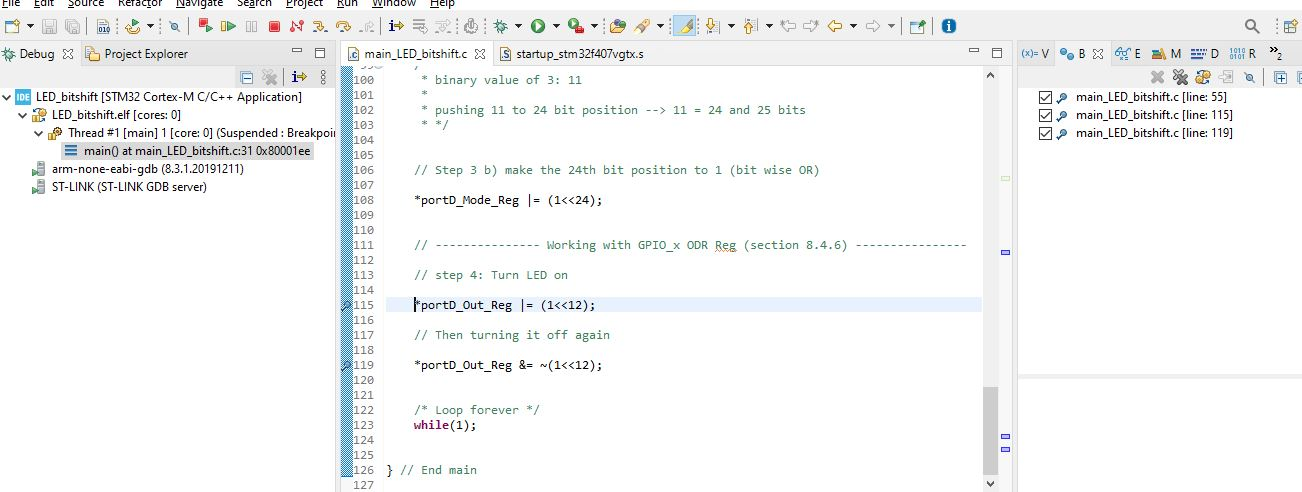
\includegraphics[scale=0.5]{Figures/driver_part_1/setting_break_point}
\caption{Setting a Breakpoint by Double-Clicking the Blue Bar Strip}
\label{fig:driver_part_1:setting_break_point}
\end{figure}

\begin{itemize}
    \item In the debug view, the right side will show a \tbi{breakpoints window}, where all the breakpoints are listed with their lines. We can deselect or remove some breakpoints from here.
\end{itemize}


    \item To go directly to the breakpoint, click on resume, as shown in \autoref{fig:driver_part_1:goto_break_point}.

  \begin{figure}[h]
\centering
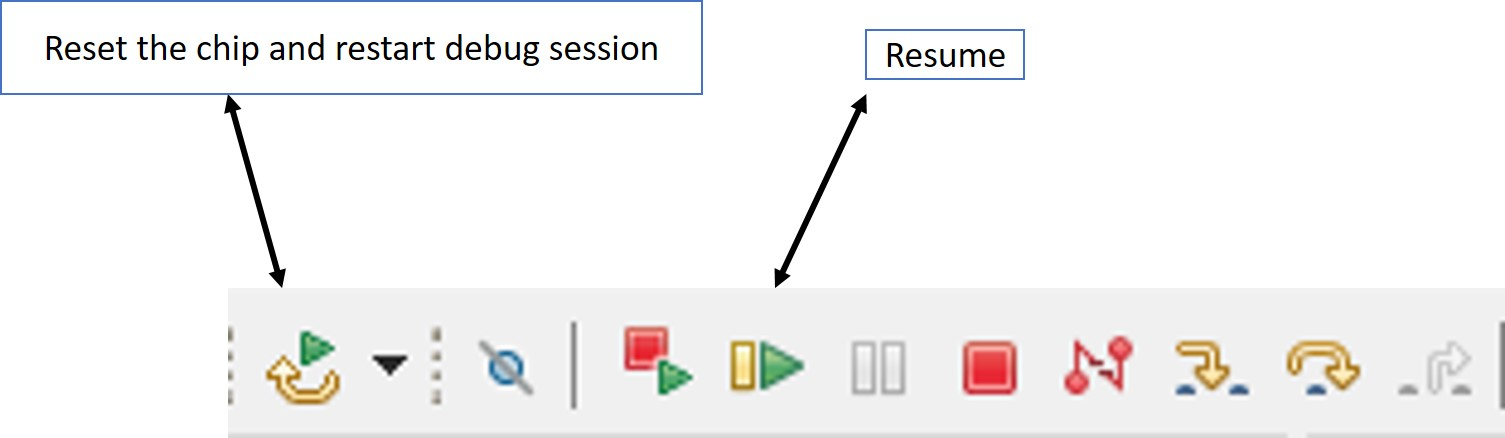
\includegraphics[scale=0.5]{Figures/driver_part_1/goto_break_point}
\caption{Going to a Breakpoint}
\label{fig:driver_part_1:goto_break_point}
\end{figure}  

\begin{itemize}
    \item To restart debugging or reset the chip, click on the reset button shown in \autoref{fig:driver_part_1:goto_break_point}.
\end{itemize}


    
\end{itemize}

\subsection{Expression Window}

The expression window is used to make real-time changes (like incrementing a variable or pointer) during a debug session. 

To use the expression window:

\begin{itemize}
    \item Start a debug session.

    \item Open the expression window by going to the \verb|Window| tab, $\rightarrow$ \verb|Show View| $\rightarrow$ \verb|Expression|. The expression window will open on the right-hand side.


    \item Drag and drop the variable from the editor: select the variable name, hold, and drag it. After this step, the variable name will appear in the expression window as shown in \autoref{fig:driver_part_1:expression_window}.


\begin{figure}[h]
\centering
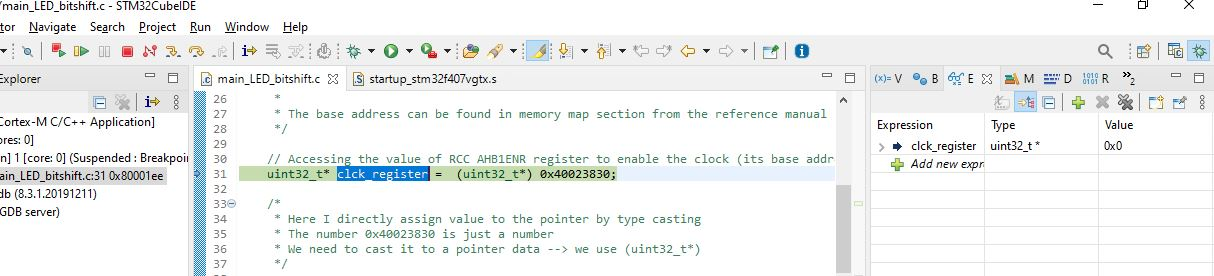
\includegraphics[scale=0.5]{Figures/driver_part_1/expression_window}
\caption{Expression Window: Dragging and Dropping a Variable}
\label{fig:driver_part_1:expression_window}
\end{figure}  

    
\end{itemize}


\subsection{Memory Window}

The memory window is used to track different memory locations in the microcontroller, such as RAM, ROM, FLASH, etc.\\

Data variables are stored in the RAM of the microcontroller.\\

\todo{Memory window:} \underline{\textit{Memory window}:} \textit{Nothing much important for now concerning addresses, maybe for later when I advance for the course material}. 


\subsection{Call Stack}

The call stack can be used to check for mistakes in our code when we don't know their source. If there is a mistake, the call stack will raise an exception, helping us identify the source of the mistake.\\

\newpage
An example of the call stack in STM32Cube IDE is shown in \autoref{fig:driver_part_1:call_stack_example}.

\begin{figure}[h]
\centering
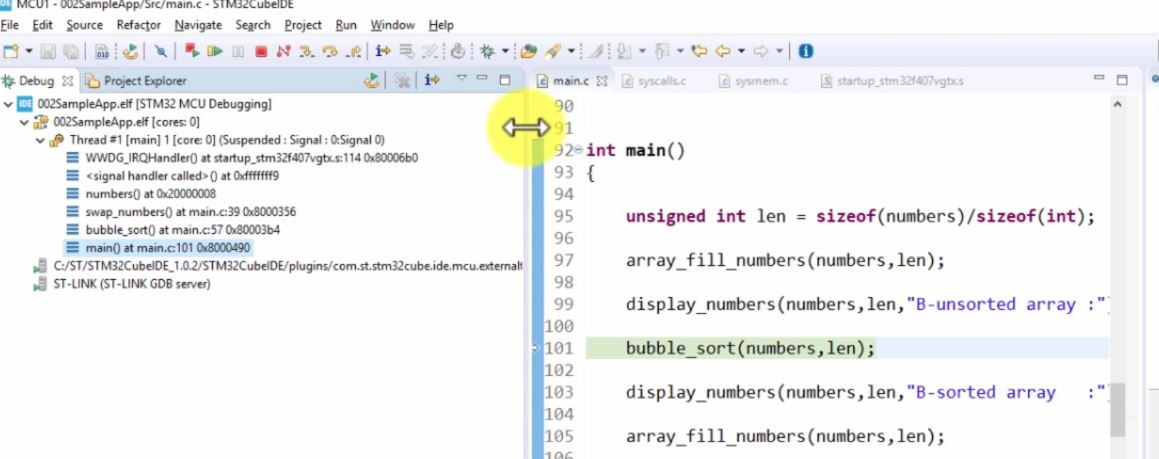
\includegraphics[scale=0.5]{Figures/driver_part_1/call_stack_example}
\caption{Call Stack Example}
\label{fig:driver_part_1:call_stack_example}
\end{figure} 

First, we see the \verb|main| function, then the \verb|bubble sort| function, and so on.\\


\todo{Call Stack} \underline{\textit{Call Stack}:} 

\begin{itemize}
    
    \item \textit{To redo it later} 

    \item \textit{To insert some mistake, and see what will happen}
    
\end{itemize}


\newpage
\subsection{Data Watchpoint}

Data watchpoints are similar to breakpoints. They detect whether the value of a variable has changed, using a debug event for detection.\\

To define a watchpoint:

\begin{itemize}
    \item Enter debug mode.

    \item Open the breakpoints window.

    \item Click on \verb|Add Watchpoints| as shown in \autoref{fig:driver_part_1:adding_watchpoints}.

\begin{figure}[h]
\centering
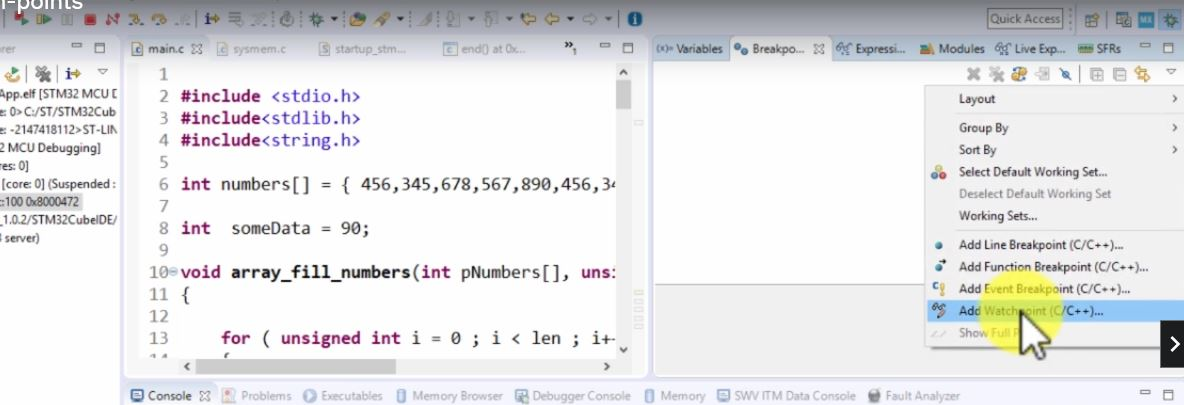
\includegraphics[scale=0.5]{Figures/driver_part_1/adding_watchpoints}
\caption{Adding Watchpoints}
\label{fig:driver_part_1:adding_watchpoints}
\end{figure} 
    
\item Add an expression (like the variable name we are trying to monitor), as shown in \autoref{fig:driver_part_1:adding_expression_name}. In this example, the variable is \verb|someData|.


\begin{figure}[h]
\centering
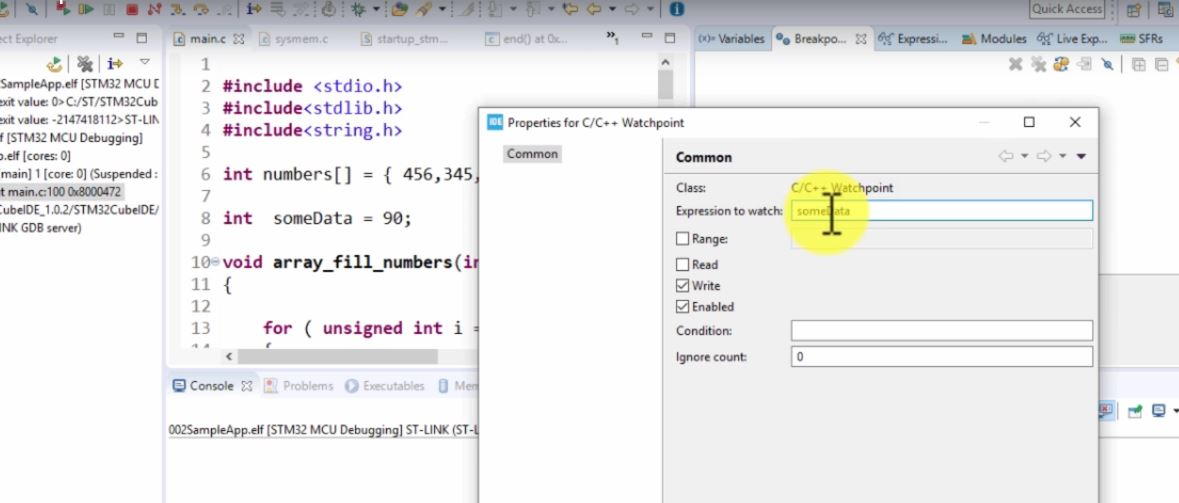
\includegraphics[scale=0.5]{Figures/driver_part_1/adding_expression_name}
\caption{Adding Expression Name to Watchpoints}
\label{fig:driver_part_1:adding_expression_name}
\end{figure} 


\end{itemize}

\todo{Data Watchpoints} \underline{\textit{Data Watchpoints}:} \textit{To repeat this part and try to see the difference between watchpoint in Read and Write mode}.


\subsection{SFR}

SFR stands for special function registers. These registers contain the configurations for the different peripherals of the microcontroller (such as timer peripherals, power, communication, etc.).\\

To view the different SFRs:

\begin{itemize}
    \item Enter debug mode.

    \item Go to the \verb|Window| tab, $\rightarrow$ \verb|Show View| $\rightarrow$ \verb|SFR|.
\end{itemize}

A screenshot of the SFR is shown in \autoref{fig:driver_part_1:SFR_microcontroller}.

\begin{figure}[h]
\centering
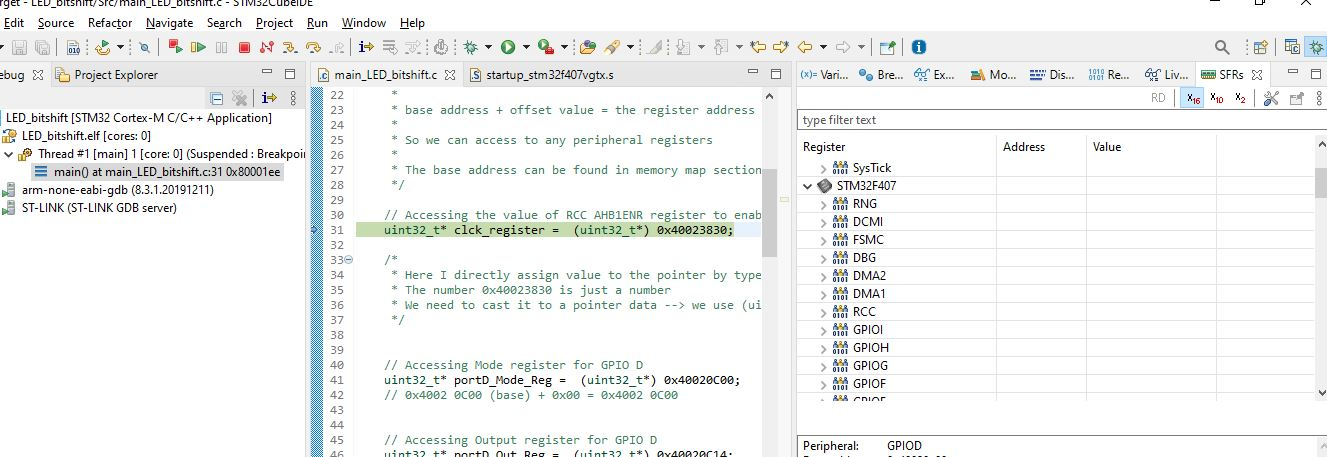
\includegraphics[scale=0.5]{Figures/driver_part_1/SFR_microcontroller}
\caption{Different SFRs of the Microcontroller}
\label{fig:driver_part_1:SFR_microcontroller}
\end{figure} 

\begin{itemize}
    \item Different SFRs for the STM32F407.
\end{itemize}

Notice that SFRs are the registers of the microcontroller. There are also some registers relative to the processor (to the ARM Cortex). These can be shown using the \verb|Window| tab, $\rightarrow$ \verb|Show View| $\rightarrow$ \verb|Registers| (and they are also shown at the top of the STM32F407 microcontroller).\\

\underline{Note:} We can also directly modify the registers using the SFR window shown in \autoref{fig:driver_part_1:SFR_microcontroller}, for example to turn on some LED as we did in \autoref{Sec:Led_practice}, but here by directly modifying the bits without writing code.


\subsection{Extra Features}

\begin{itemize}
    \item List all functions implemented in the \verb|main| (to avoid scrolling too much): \verb|Ctrl + o|.


    \item In debug mode, we can run the code on the MCU using the run button as shown in \autoref{fig:driver_part_1:goto_break_point}.

    \begin{itemize}
        \item Once the code is running, the resume button will not be highlighted anymore.

        \item If we want to stop the execution, we click on the suspend button (next to the resume button).
    \end{itemize}


    \item To enable autocomplete and code proposals, press left \verb|Ctrl|+ space.

    \item To edit some code in a debug session without closing the debug and rebuild (to automate tasks):

    \begin{enumerate}
        \item Switch from debug view to editing mode. 

        Add the necessary code.

        \item Click on terminate and relaunch (icon shown in the IDE).


        This will rebuild, download the code, and switch the debug perspective. 
    \end{enumerate}

    
\end{itemize}


\newpage
\section{MCU Memory Map}

This section describes how to fetch the corresponding addresses of each peripheral (GPIOx, timer, etc.).\\


\underline{Note:} Most information in this section is described back in \ref{Sub:Hardware_GPIO_Bus} and \ref{Sub:Peripheral_Information}. Review them if you need more information.


\section{MCU Bus Interface}

\tbi{When fetching the address of some peripheral, we need to know to which bus it is connected}. Also, buses play an important role in communication between several peripherals of the MCU. 

In this section, we present several buses used in the MCU.\\

\underline{Note:} The bus information is relevant to the processor vendor (ARM in our case), and we need to refer to the ARM documentation (such as the ARM technical reference manual).\\


In \autoref{fig:driver_part_1:bus_block_diagram_cortex_flash}, we have the block diagram where we have 3 buses between the Cortex M4 processor and the FLASH.

\underline{Note:} \autoref{fig:driver_part_1:bus_block_diagram_cortex_flash} is from the data sheet, section 2.2.


\begin{figure}[h]
\centering
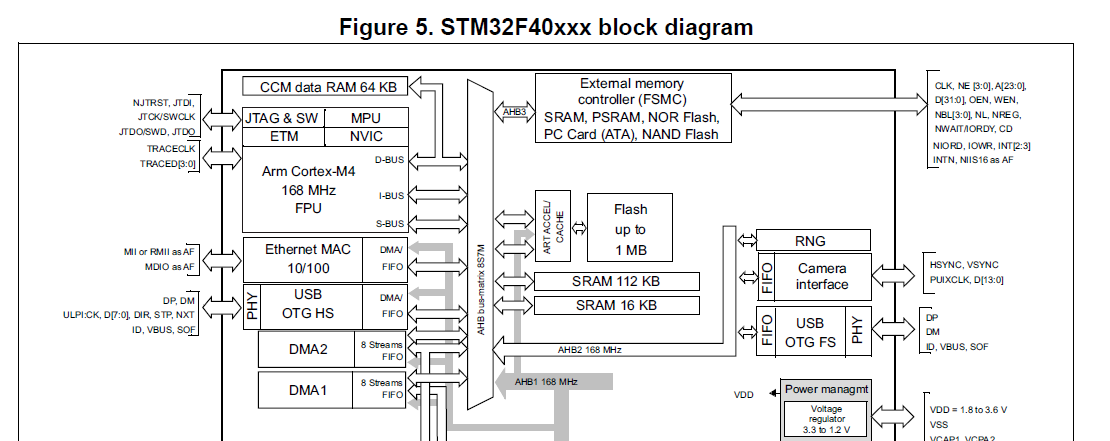
\includegraphics[scale=0.8]{Figures/driver_part_1/bus_block_diagram_cortex_flash}
\caption{Bus between Cortex M Processor and FLASH}
\label{fig:driver_part_1:bus_block_diagram_cortex_flash}
\end{figure} 

\begin{itemize}
    \item I bus: for instruction.

    \item D bus: for data.

    \item S bus: called system bus.
\end{itemize}

\newpage
Suppose we have some code as shown in \autoref{fig:driver_part_1:some_code_example_1}.

\begin{figure}[h]
\centering
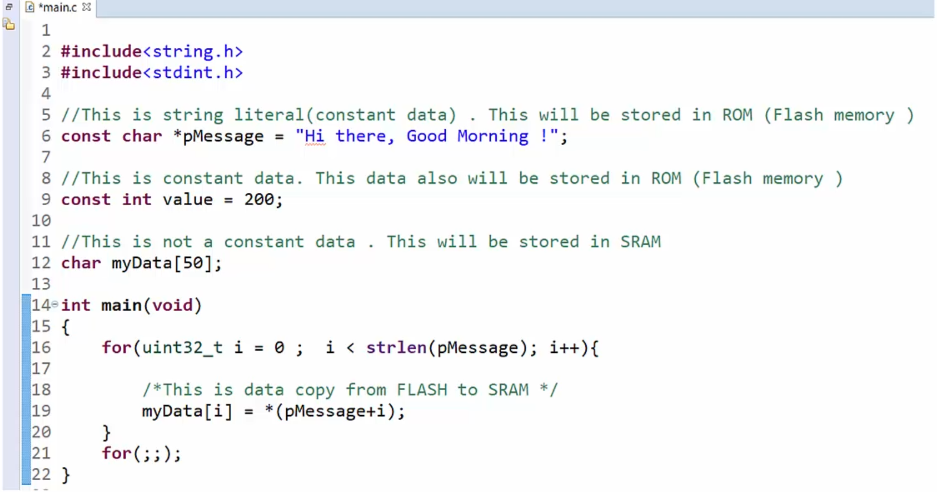
\includegraphics[scale=0.7]{Figures/driver_part_1/some_code_example_1}
\caption{Some Code Example}
\label{fig:driver_part_1:some_code_example_1}
\end{figure} 

\begin{itemize}
    \item Constant data is stored in FLASH.

    \item The variable data is stored in SRAM.
\end{itemize}

When we compile and download the code, the processor reads the instruction from the FLASH using the I bus, and the constant data using the D bus from FLASH.\\

\underline{Note:} We know that the I and D buses are connected to the FLASH from the reference manual, as shown in \autoref{fig:driver_part_1:I_D_bus_to_FLASH}.

\begin{figure}[h]
\centering
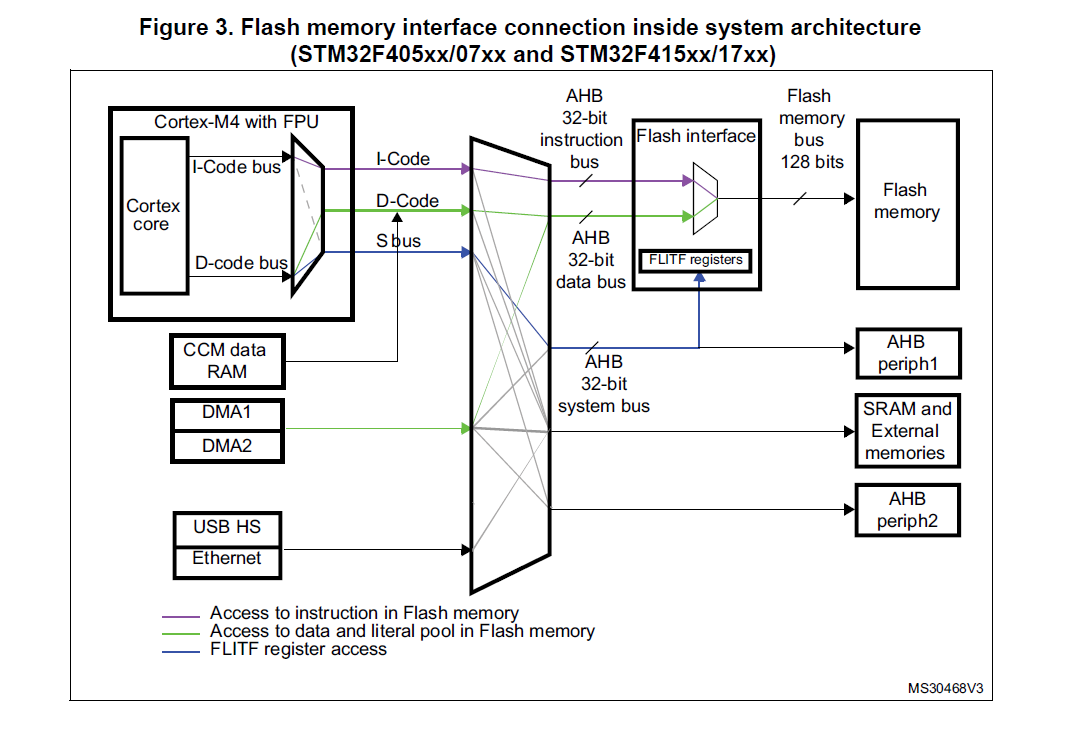
\includegraphics[scale=0.7]{Figures/driver_part_1/I_D_bus_to_FLASH}
\caption{I and D Bus Connected to FLASH}
\label{fig:driver_part_1:I_D_bus_to_FLASH}
\end{figure} 


To know more about these buses, we use the \textit{ARM Cortex M4 Technical Reference Manual r0p1}, and refer to section 2.3: Interfaces.

From this manual, we can see that each bus has a specific operating address range. For example, the ARM Cortex uses the I bus to fetch instructions that are within the range  0x00000000 to 0x1FFFFFFC. The same concept applies to the D bus and system bus.


\subsection{Bus Matrix}

One last thing to explain is the bus matrix. In \autoref{fig:driver_part_1:bus_matrix}, we have a diagram illustrating the concept of the bus matrix.

\begin{figure}[h]
\centering
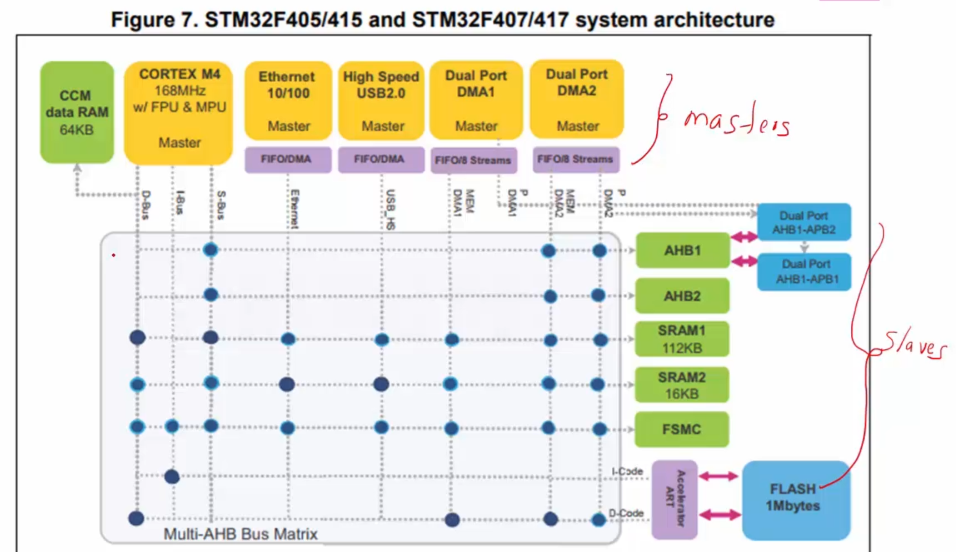
\includegraphics[scale=0.7]{Figures/driver_part_1/bus_matrix}
\caption{Illustrating Bus Matrix}
\label{fig:driver_part_1:bus_matrix}
\end{figure} 

\begin{itemize}
    \item In the MCU, the communication between the processor and other peripherals is based on a Master-Slave model.

    \item The dots indicate possible communication paths.

    \item For example, the Cortex M4 can communicate with four peripherals using the D bus (as we have four dots): SRAM 1 and 2, FSMC, and the FLASH.

    \item Notice that we can't communicate between the S bus of the Cortex and FLASH since we don't have a dot.
    
\end{itemize}


Also, concerning the bus matrix, by observing \autoref{fig:driver_part_1:some_code_example_1}, we can see that the bus matrix is extended to the \verb|AHB1| bus, then continues until we have a conversion from \verb|AHB| $\rightarrow$ \verb|APB|, but with lower speed. 

\newpage
\section{Clocks in MCU}

Now we begin with clocks. MCUs are essentially \tbi{digital synchronous circuits}. By synchronous, we mean they operate in sync with a clock: we can't do anything if we don't have some clock source.\\

Usually, we have three types of clock sources in any MCU:

\begin{enumerate}
    \item Crystal oscillator: an external circuit that provides the clock.

    \begin{itemize}
        \item Also called HSE (high-speed external).
    \end{itemize}

    \item RC oscillator: internal circuitry inside the MCU.

    \begin{itemize}
        \item Called HSI: stands for high-speed internal.
    \end{itemize}

    \item PLL: provides a high-frequency clock from lower frequencies (also an HSI).
\end{enumerate}


\underline{Design Criteria:} Choosing the clock frequency is important for low-power applications, as there is usually a relation between frequency and power consumption.

\todo{frequency and power relation} \underline{\textit{Frequency and Power Relation}:} \textit{To be explored later}.\\

For the MCU discovery board, we have an 8 MHz clock, coming from an installed crystal oscillator (which can be viewed in the schematic, called \verb|X2|). In the Nucleo board, we don't have an installed crystal oscillator like the discovery family board, but we can \textit{extend one} from the ST-Link circuitry.


\underline{Notes:}

\begin{itemize}
    \item See the hand notes I wrote in the reference manual, section 6.2, Figure 16: clock tree.

    \item The PLL, in general, boosts the clock speed beyond the limits of HSE and HSI.

    \item Some peripherals, such as Ethernet, won't work properly if we underclock them, so we need to use a PLL.
\end{itemize}

To configure the clock, we need to use the \verb|RCC| register (description of this full register is in section 6.3 of the reference manual). Using \verb|RCC|, we can configure various domains such as \verb|AHB|, \verb|APB|, memory domain, etc.\\

\underline{Some Rules Regarding Clocks:}

\begin{itemize}
    
    \item In programming, and before using any peripheral, we need to configure the clock associated with the peripheral.

    \item By default, the clocks are in sleep mode to save power.

    \item To know the corresponding clock for a peripheral, we need to know the bus associated with this peripheral.

    \begin{itemize}
        \item For that, we can use the memory map table in the reference manual (section 2.3, Table 1), or use the functional overview (the block diagram) from the data sheet (section 2.2, figure 5).
    \end{itemize}
    
\end{itemize}

\todo{ADC Configuration Ex} \underline{\textit{ADC Configuration Ex}:} \textit{To see the code later, take a screenshot. Nice way of using MACROS.}

\newpage

\subsection{HSI Measurement Exercise}

In this part, we will try to code an exercise to measure an HSI clock.\\

\underline{Given:}

\begin{itemize}
    \item Write a program to output the HSI clock on an MCU pin and measure it using an oscilloscope or logic analyzer.
\end{itemize}

Steps to output a clock to an MCU pin:

\begin{enumerate}
    \item Select the desired clock for the MCOx signal (stands for MC Clock Output). 

    \begin{itemize}
        \item We need to use the \verb|RCC-CFGR| register (section 6.3.3 from the reference manual).
    \end{itemize}

    \item Output the signal to the MCU pin.

    \begin{itemize}
        \item For the pin, we need to refer to the data sheet.

        \item Go to chapter 3, table 1 for alternate function.

        \item By alternate function, we mean that a port can be used for several different functions. 

        \item In our case, \verb|MCO1| will be used by GPIO \verb|PA8| such that \verb|PA8| is in \verb|AF0| mode.

        
    \end{itemize}
    
\end{enumerate}      

\underline{Note:} If we want to know \verb|PA8| as a pin number, we can look at the board schematic: \verb|PA8| $\leftrightarrow$ pin 67.\\ 

\underline{Logic Analyzer and Board Connection:} See video 39.\\

In \autoref{fig:driver_part_1:logic_analyzer_MCU_connection}, we have a block diagram to make the connection.


\begin{figure}[h]
\centering
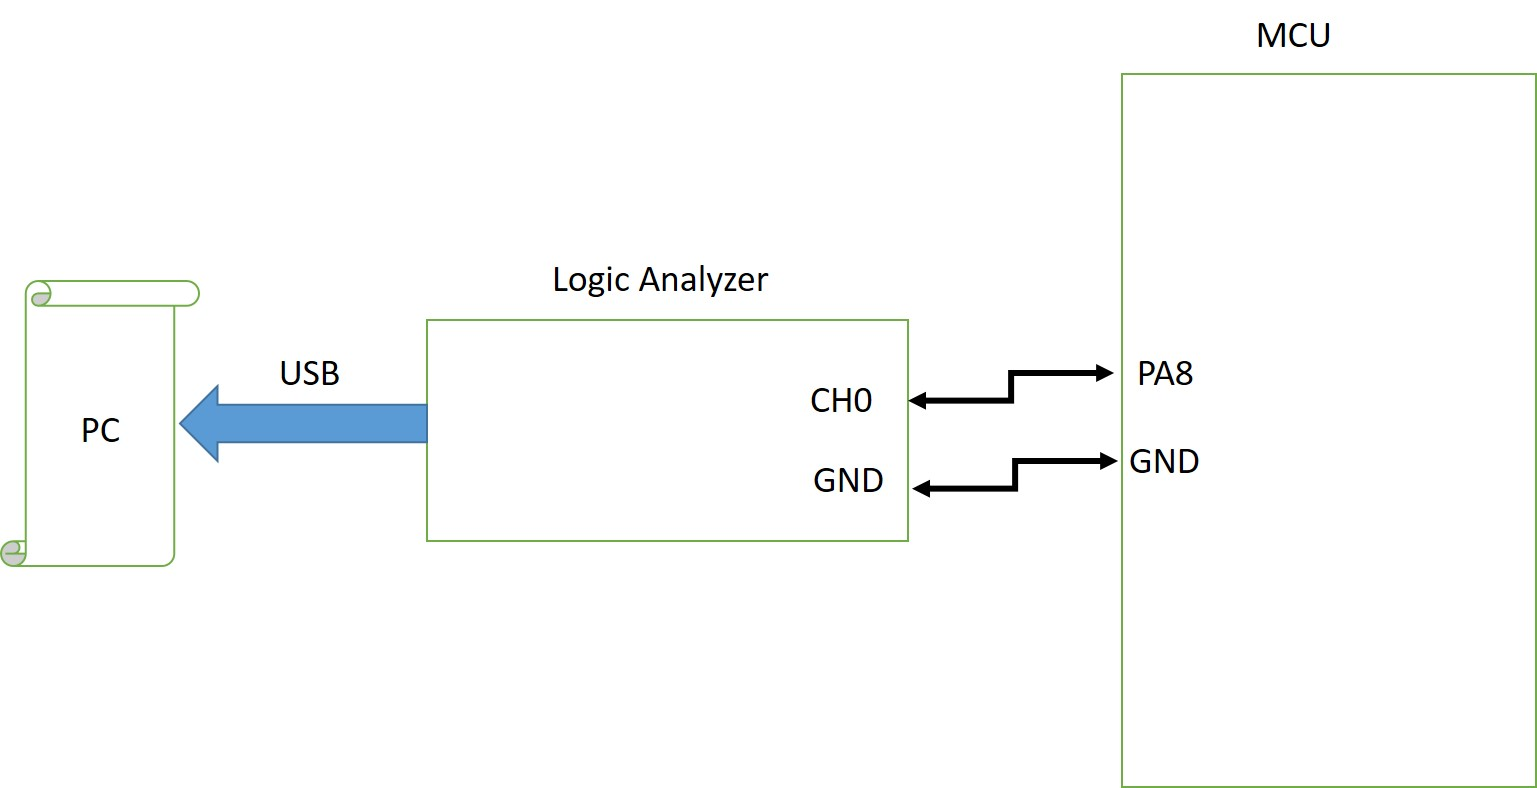
\includegraphics[scale=0.5]{Figures/driver_part_1/logic_analyzer_MCU_connection}
\caption{Connection between Logic Analyzer and MCU}
\label{fig:driver_part_1:logic_analyzer_MCU_connection}
\end{figure} 


\todo{Code Clock Measurement} \underline{\textit{Code Clock Measurement}:} \textit{To be done later, when buying the logic analyzer (See video 40 and 41)}. 


\newpage

\section{Vector Table}

\underline{Resources:} Refer to chapter 12 in \cite{book_Embedded_systems_ARM_Cortex_M_YifengZhu} , and table 61 in the reference manual.\\

\underline{Naming and Definition:}\\

The vector table is a table that contains the addresses of interrupts and system exceptions (review \autoref{chap:arm_cortex} to get more details about interrupts and system exceptions).\\

The name vector usually stands for direction in mathematical terms. Here, in embedded programming, the direction is equivalent to pointers, which hold addresses; hence the name vector table since it is a table of addresses.\\ 

We try to explain all its columns:

\begin{itemize}
    \item Position: it is also the IRQ number with respect to NVIC position
    
    	\begin{itemize}
    	\item Note that for system exceptions, we don't have numbers since the MCU vendor don't have a choice in designing them
    	
    	\item It is the processor manufacturer (ARM in this case) which has the choice, since the system exceptions are internal (from inside the processor)
    	\end{itemize}

    \item Priority: priority which comes first from the handler. By default, the less the number, the more prior it is.

    \item Type of Priority: 

    \begin{itemize}
        \item Fixed: we can't change it using code.

        \item Settable: we can change it using code. Here, we can change the priority: make some handler which is by default less prior, more prior.
    \end{itemize}


    \item Addresses: place to store the function which implements the interrupt. In other words, if we implement a function NMI, this function accepts the address \verb|0x00000008| 
    
    Example:

    \begin{itemize}
        \item 0x 0000 0008 holds the function implementing the NMI handler.
    \end{itemize}

    \todo{interrupt and function pointer} \underline{\textit{Interrupt and Function Pointer}:} \textit{To review the concept of function pointer later and document it all}.

    As another example: take for example \verb|I2C1| event interrupt. This will be a normal function contained in the startup file (having a \verb|.s| extension). 
    
    This function is stored in a certain address (say for example 0x8000264). By referencing the table, we see that \verb|I2C1| has 0x0000 00BC. This means when the processor activates the \verb|I2C1|, it goes to 0x0000 00BC which contains 0x8000264.
    
    
\end{itemize}


\todo{Vector Table} \underline{\textit{Vector Table}:} \textit{This is more explained in chapter 2: embedded programming using Cortex M. To redo it then get back to the video of this section (video 42)}. 

\subsection{Startup and Linker Script}

\begin{itemize}

\item In the MCU IDE, the interrupt and system exceptions are handled in the startup file, inside the startup folder.


\item The vector table, for example, is coded as a big array of constants named \verb|isr_vector|.

\item The \verb|isr_vector| is stored in the linker script (with \verb|.ld| extension, inside the ROM, see line 54 in \verb|STM32F407VGTX_FLASH.ld| file).
 
\end{itemize}

\todo{linker and startup:} \underline{\text{Linker and Startup}:} \text{To be explored later in the ARM processor course.}

\newpage
\section{Programming: User Button Interrupt}

In this section, we apply the concept of interrupt by using the button attached to our MCU.

\subsection{Button Location in MCU}

$\mathrm{1}^\mathrm{st}$, we open the user \textit{user manual} in order to know how the button interacts with our MCU.

We go to figure 16 (peripherals) in the figure labeled user and wake button (it is also shown in \autoref{fig:driver_part_1:push_button_schematic})

\begin{figure}[h]
\centering
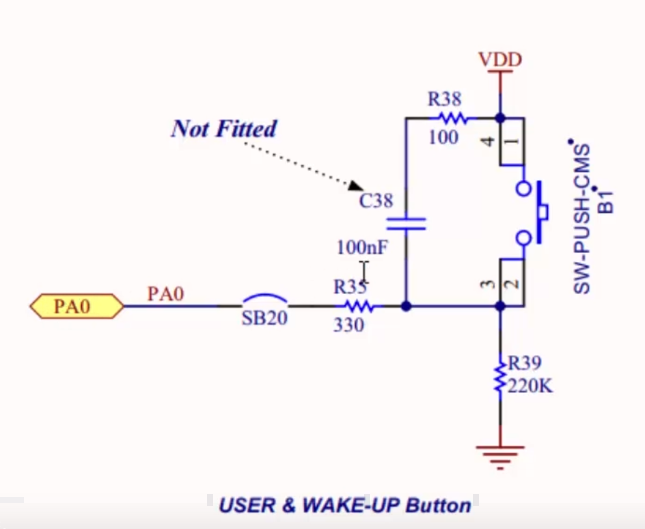
\includegraphics[scale=0.5]{Figures/driver_part_1/push_button_schematic}
\caption{Connection between Logic Analyzer and MCU}
\label{fig:driver_part_1:push_button_schematic}
\end{figure}

	\begin{itemize}
	
	\item The capacitor C38 marked \textit{not fitted}: meaning if it is like it doesn't exist.
	
	\item When we push the button, we have a big resistance R39 compared to R35 $\rightarrow$ PA0 will be pulled to VDD $\leftrightarrow$ a high state
	
	\item When we release the button, the easiest path is to ground $\rightarrow$ it will be in a low state.
		
	
	\end{itemize}

Before implementing, we need to understand many concepts related to this task.

\subsection{GPIO Interrupts}

Now the next step is to see how GPIO interrupts are delivered to the processor. This task is \tbi{vendor specific}.

For that, we go to the \textit{reference manual}, section 12.2 (external interrupt/event controller) EXTI.

In \autoref{fig:driver_part_1:exti_gpio_mapping}, we have the mapping for each GPIO pin and EXTI engine. 

\begin{figure}[h]
\centering
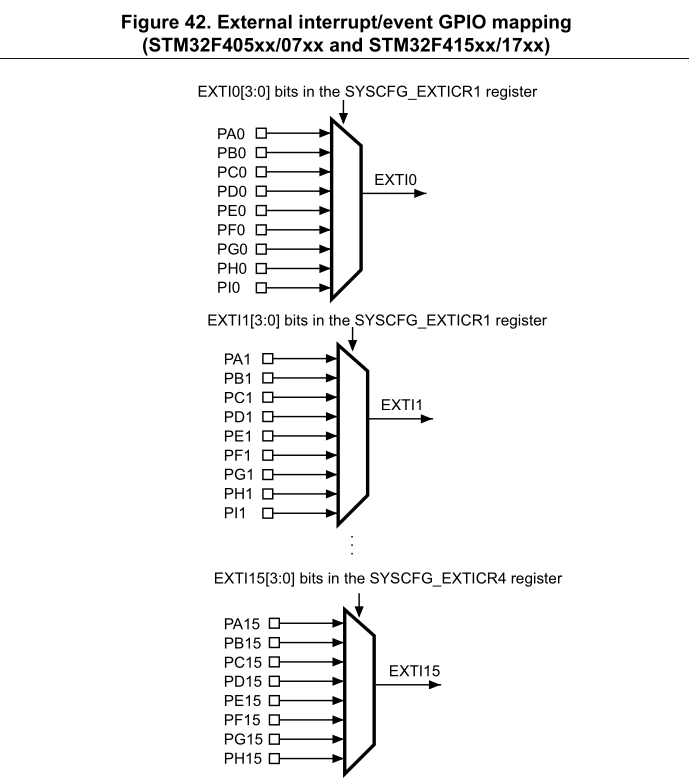
\includegraphics[scale=0.5]{Figures/driver_part_1/exti_gpio_mapping}
\caption{EXTI and GPIO Mapping}
\label{fig:driver_part_1:exti_gpio_mapping}
\end{figure}


\newpage
\section{Summary: Driver Part 1}

\begin{itemize}


\item \underline{Design Criteria:} Choosing the clock frequency is important if we want to work in low-power applications, since usually there is a relation between frequency and power consumption.

\item \underline{Some Rules Regarding Clocks:}

\begin{itemize}
    
    \item In programming, and before using any peripheral, we need to configure the clock associated with the peripheral.

    \item By default, the clocks are in sleep mode to save power.

    \item To know the corresponding clock for a peripheral, we need to know the bus associated with this peripheral.

    \begin{itemize}
        \item For that, we can use the memory map table in the reference manual (section 2.3, Table 1), or use the functional overview (the block diagram) from the data sheet (section 2.2, figure 5).
    \end{itemize}
    
\end{itemize}

\item Interrupt resources: see 

\end{itemize}